\documentclass[tikz]{standalone}

\usepackage[latin1]{inputenc}
\usepackage{tikz}

% GNUPL
\begin{document}
\pagestyle{empty}
\newcommand\spiral{}% Just for safety so \def won't overwrite something
\def\spiral[#1](#2)(#3:#4:#5){% \spiral[draw options](placement)(end angle:revolutions:final radius)
\pgfmathsetmacro{\domain}{pi*#3/180+#4*2*pi}
\draw [#1,shift={(#2)}, domain=0:-\domain,variable=\t,samples=int(\domain/0.08)] plot ({\t r}: {#5*\t/\domain})
}
\def\spirall[#1](#2)(#3:#4:#5){% \spiral[draw options](placement)(end angle:revolutions:final radius)
\pgfmathsetmacro{\domain}{pi*#3/180+#4*2*pi}
\draw [#1,shift={(#2)}, domain=0:\domain,variable=\t,samples=int(\domain/0.08)] plot ({\t r}: {#5*\t/\domain})
}

\usetikzlibrary{decorations.pathreplacing,decorations.markings,arrows}
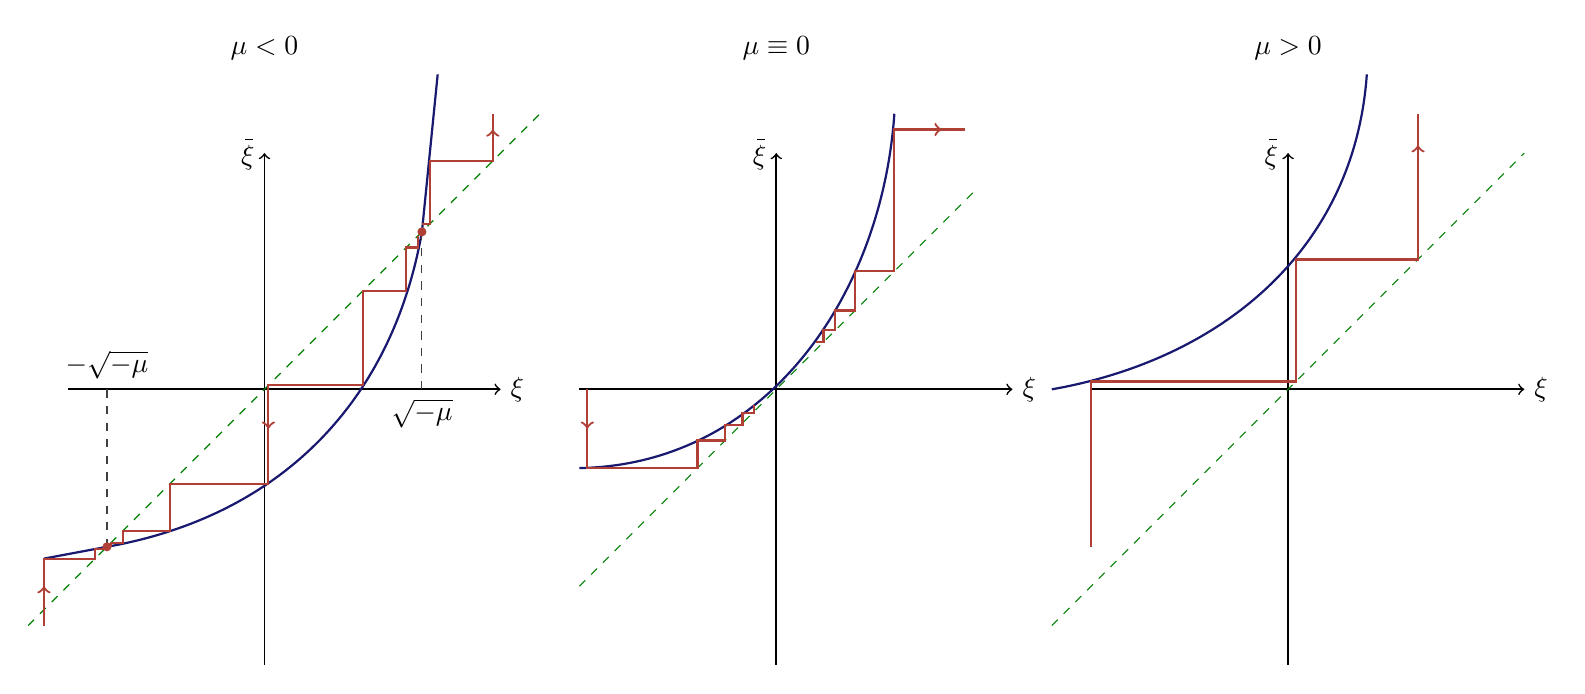
\begin{tikzpicture}
    %\mu<0
    \coordinate [label=-90:$\mu<0$] (8) at (3,8.6);

    \draw[semithick] [->] (0.5,4) -- (6,4) node[right] {$\xi$};
    \draw[semithick] [->] (3,0.5) -- (3,7) node[left] {$\stackrel{\_}{\xi}$};
    % \draw [black, semithick, domain=0:6,samples=200] plot (\x,  {1+0.2*(\x)^2+0.05*(\x)});
    \draw [color={rgb,255:red,25; green,25; blue,112},thick] (0.2, 1.85) -- (1,2) to [out=10,in=-100] (5,6) --(5.2, 8);
    \draw [black, dashed, color={rgb,255:red,0; green,128; blue,0},] (0,1) -- (6.5, 7.5);
    \draw [black, dashed, darkgray] (5,4) -- (5,6);
    \draw [black, dashed, darkgray] (1,4) -- (1,2);
    \coordinate [label=90:$-\sqrt{-\mu}$] (8) at (1,4);
    \coordinate [label=-90:$\sqrt{-\mu}$] (8) at (5,4);
    \draw [thick,color={rgb,255:red,176; green,63; blue,53}] (0.2,1) -- (0.2, 1.85) -- (0.85, 1.85) --(0.85,1.97) -- (0.97, 1.97);
    \draw[thick, color={rgb,255:red,176; green,63; blue,53}] [->] (0.2,1) -- (0.2, 1.5);
    \draw [fill, color={rgb,255:red,176; green,63; blue,53}] (1,2) circle [radius=0.05];
    \draw [color={rgb,255:red,176; green,63; blue,53},thick] (1.05,2) -- (1.05,2.05) -- (1.2, 2.05) -- (1.2,2.2) -- (1.8,2.2) -- (1.8,2.8) --(3.05,2.8) --(3.05,4.05) -- (4.25, 4.05) -- (4.25, 5.25) -- (4.8,5.25) -- (4.8,5.8) -- (4.95,5.8) -- (4.95, 5.95);
    \draw [fill,color={rgb,255:red,176; green,63; blue,53}] (5,6) circle [radius=0.05];
    \draw [color={rgb,255:red,176; green,63; blue,53},thick] [->] (3.05,3.8) --(3.05,3.5);
    \draw [color={rgb,255:red,176; green,63; blue,53},thick] (5.,6.1) -- (5.1,6.1) -- (5.1,6.9) -- (5.9,6.9) -- (5.9,7.5);
    \draw [color={rgb,255:red,176; green,63; blue,53},thick] [->] (5.9,6.9) -- (5.9,7.3);
	%\mu=0
    \coordinate [label=-90:$\mu \equiv0$] (8) at (9.5,8.6);

    \draw[semithick] [->] (7,4) -- (12.5,4) node[right] {$\xi$};
    \draw[semithick] [->] (9.5,0.5) -- (9.5,7) node[left] {$\stackrel{\_}{\xi}$};
    \draw [black, dashed, color={rgb,255:red,0; green,128; blue,0},] (7,1.5) -- (12, 6.5);
    \draw [color={rgb,255:red,25; green,25; blue,112},thick] (7, 3) to [out=1,in=-94] (11,7.5);
    % \draw [fill,color={rgb,255:red,176; green,63; blue,53}] (9.5,4) circle [radius=0.05];
    \draw [color={rgb,255:red,176; green,63; blue,53},thick] (7.1,4) -- (7.1,3)--(8.5,3) -- (8.5,3.35) -- (8.85,3.35) -- (8.85,3.55)--(9.07,3.55)--(9.07,3.7) -- (9.22,3.7) -- (9.22,3.8);
    \draw [color={rgb,255:red,176; green,63; blue,53},thick] [->] (7.1,3.8) -- (7.1,3.5);
    \draw [color={rgb,255:red,176; green,63; blue,53},thick] (10,4.6) -- (10.1,4.6) -- (10.1,4.75)--(10.25,4.75) --(10.25,5)--(10.5,5) -- (10.5, 5.5) -- (10.7, 5.5) -- (11,5.5) --(11,7.3) -- (11.9, 7.3);
    \draw [color={rgb,255:red,176; green,63; blue,53},thick] [->] (11.4, 7.3) -- (11.6, 7.3);
    %\mu>0
    \coordinate [label=-90:$\mu>0$] (8) at (16,8.6);

    \draw[semithick] [->] (13.5,4) -- (19,4) node[right] {$\xi$};
    \draw[semithick] [->] (16,0.5) -- (16,7) node[left] {$\stackrel{\_}{\xi}$};
    \draw [black, dashed, color={rgb,255:red,0; green,128; blue,0},] (13,1) -- (19, 7);
    \draw [color={rgb,255:red,25; green,25; blue,112},thick] (13, 4) to [out=10,in=-94] (17,8);
    \draw [color={rgb,255:red,176; green,63; blue,53},thick] (13.5,2) -- (13.5,4.1) -- (16.1,4.1) -- (16.1,5.65) -- (17.65,5.65) -- (17.65,7.5);
    \draw [color={rgb,255:red,176; green,63; blue,53},thick] [->] (17.65,7) -- (17.65,7.1);
\end{tikzpicture}


\end{document}